\setcounter{page}{1}
\chapter{INTRODU\c{C}\~AO}  %%Nesta linha, dentro de { }, digita-se em CAIXA ALTA, como apresentado aqui
\label{chap:01}
A engenharia de \textit{software} surgiu como um esforço de aplicar processos que pudessem dar maior assertividade nos projetos de \textit{software}. Através desses esforços surgiram vários modelos que contribuíram para melhorar o cenário de desenvolvimento. Pode-se dizer que esses esforços foram também impulsionados através do mercado, o qual se torna cada vez mais competitivo e exige que os projetos de \textit{software} tenham que ser desenvolvidos com extrema qualidade e de forma rápida, repetida e confiável.
Dentre as várias metodologias que surgiram, uma metodologia está ganhando bastante destaque no mercado atual: o \textit{lean}. \citeonline{4222727} aponta que iniciativas \textit{lean} (ou enxuta)\footnote{Neste trabalho é empregado a palavra em inglês lean.}  tem sido utilizadas com sucesso em vários setores como manufatura, logística, serviços e no desenvolvimento de produtos, a fim de garantir uma melhor entrega no que tange ao custo, qualidade e prazo. Uma pergunta que surge naturalmente é: “É possível aplicar os mesmos conceitos já aplicados em outros setores para o \textit{software} ?”. Esse trabalho propõe-se a responder essa e outras perguntas sobre aplicação do \textit{lean} no contexto de \textit{software}.
Na seção seguinte, são mostrados alguns trabalhos na linha de pesquisa do \textit{lean} e que contribuíram para o trabalho.

\section{TRABALHOS RELACIONADOS}

No trabalho  de \citeonline{4222727} é mostrado um breve tutorial para aplicação de \textit{lean} no desenvolvimento de \textit{software}. O \textit{lean} é focado em sete princípios:

\begin{itemize}
	\item Eliminar desperdício;
	\item Incorporar qualidade;
	\item	Criar conhecimento;
	\item	Adiar compromisso;
	\item	Entregar rápido;
	\item	Respeitar pessoas e
	\item	Otimizar o todo.
\end{itemize}

Todo esse grupo de princípios, segundo esse trabalho, fornece uma orientação de como entregar um \textit{software} de forma rápida, melhor e com um custo menor. Neste trabalho é afirmado que o desenvolvimento de \textit{software lean} fornece a teoria por trás das práticas utilizadas pelo desenvolvimento ágil. Além disso, o \textit{lean} fornece para as empresas uma série de princípios para melhorar o processo de engenharia de software com a finalidade de trazer melhora no contexto do cliente, domínio do negócio, capacidade de desenvolvimento e em uma eventual situação única que a empresa enfrente.

Neste trabalho, um tutorial foi feito com uma turma e a aplicabilidade do \textit{lean} no desenvolvimento de \textit{software} é feita através dos seus princípios fundamentais. No princípio do desperdício, além de sua explicação no contexto de \textit{lean}, foi mostrado como enxergar o desperdício no contexto do desenvolvimento e explanado os sete desperdícios no desenvolvimento de \textit{software}. Nesta etapa, a classe foi divida em grupos de até sete pessoas e foi feito um mapeamento de fluxo de valor da experiência de alguém no grupo. Após a elaboração, os grupos apresentaram seu mapa e receberam críticas dos outros participantes.

Para o próximo conceito do \textit{lean}, qualidade, foram apresentados conceitos como: TDD (\textit{test-driven development}), teste unitário automatizado e teste de aceitação. Essa etapa não focou muito em como fazer, mas o porquê da importância dessas práticas para o \textit{lean}\textit{.}

Uma análise racional, no que se refere ao conhecimento, foi feita sobre a questão de postergar os compromissos (princípio do pensamento \textit{lean}). Também foram apresentados métodos que visam preservar o conhecimento de forma que os times não tenham que reaprender o que já foi aprendido. Além disso, foi feita uma discussão dos benefícios da utilização de uma abordagem que envolve explorar múltiplas soluções em vez de focar em apenas uma.

Para questão de velocidade é discutido a aplicação da teoria das filas no desenvolvimento de \textit{software}. Nela foi mostrado o porquê de longas filas serem prejudiciais ao desenvolvimento e mostrado como evita-las. Além disso, é mostrado que ciclos de vida rápidos tendem a dar uma qualidade maior ao projeto de \textit{software} e reduzir seu custo.

Por fim, foi discutido a importância de enxergar um sistema como um todo. Através dessa discussão foi explanado que não é suficiente focar apenas no desenvolvimento em si, assim foi mostrado como mudar o foco do desenvolvimento para os esforços dos objetivos em geral, ou seja, o produto ou o processo apoiado pelo \textit{software}. 

A abordagem de migração para o \textit{lean} de uma empresa de \textit{software}, no trabalho de \citeonline{7107412}, também foi feita a partir da medição do fluxo de valor da organização com posterior utilização desses dados para migração. Essa equipe já utilizava a metodologia ágil de desenvolvimento. Para medir o fluxo de valor, são medidos aspectos de interesse das atividades, recursos utilizados e artefatos produzidos. É importante notar que, como assinala \citeonline{7107412}, o que é de interesse do ponto de vista para os objetivos de uma empresa não necessariamente é para outra. Por isso é utilizado a estratégia GQM+ (\textit{Goal Question Metric Plus}). A estratégia GQM+ é uma nova abordagem de medida baseada no GQM (\textit{Goal Question Metric}). A diferença segundo \citeonline{DBLP:journals/corr/BasiliHLMRRST14} é que o GQM+ alinha as medidas do \textit{software} com os objetivos da empresa. Essa abordagem foi necessária a fim de ajudar na correspondência das estratégias com a necessidade de informação e medidas. Os dados obtidos são usados para entender melhor o processo de desenvolvimento de \textit{software}. Uma técnica chamada Andon é então utilizada no sentido de fornecer um mecanismo para visualização dos dados por qualquer pessoa com o menor esforço possível. Através desse mecanismo de visualização, um feedback para o time é feito no sentido de guia-los nos seus objetivos. Na figura \ref{fig:01} é mostrado um mapa que ilustra a dinâmica do \textit{lean} em uma empresa que emprega o processo de desenvolvimento ágil.

\begin{figure}[hb]
\begin{center}
\caption{Mapas de conceito descrevendo os blocos de construção do desenvolvimento de software lean}
\label{fig:01}
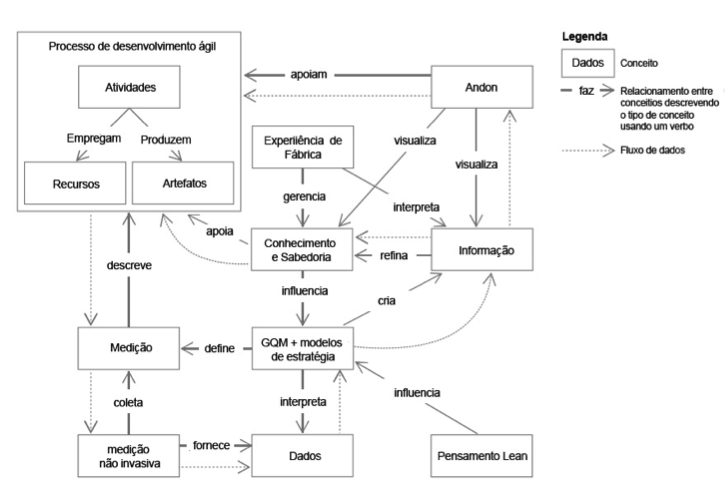
\includegraphics[width=15cm]{assets/figura1} \\
\fonte{Adaptado de \citeauthoronline{7107412}, \citeyear{7107412}.}
\end{center}
\end{figure}

Na Figura \ref{fig:01} obverva-se que o processo de desenvolvimento ágil possui atividades, as quais utilizam-se de recursos e produzem artefatos. É possível perceber também que o processo do \textit{lean} não está associado unicamente ao processo de desenvilmento da organização. Por essa razão a abordagem GQM+ foi um diferencial. Através de um sistema de retroalimentação, tem-se um \textit{feedback} que contribui também para melhora contínua do sistema como um todo.

O trabalho de \citeonline{6005500} foca na combinação do \textit{lean} com metodologias ágeis, como o trabalho de \citeonline{7107412}. \citeonline{6005500} afirma que existem linhas de pesquisa que consideram que ágil e o \textit{lean} são dois nomes para mesma coisa, enquanto outras linhas consideram que não. Os autores que consideram que \textit{lean} e ágil não são a mesma coisa possuem basicamente duas visões: a de que \textit{lean} e ágil estão em níveis diferentes dentro da organização e outra que afirma que \textit{lean} e ágil possuem diferentes focos e escopos. \cite{6005500}

% Para algumas linhas de pesquisa, as duas metodologias tem o mesmo objetivo, mas estratégias diferentes. O \textit{lean} nasceu de uma filosofia de gerenciamento que foca nos seus princípios, e.g. eliminação de atividades que não agregam valor ao cliente, não apenas dentro do gerenciamento da organização como em toda cadeia (o que inclue o desenvolvimento). Nesse sentido, pode-se afirmar que sua aplicabilidade dentro da organização segue uma abordagem \textit{top-down}, ou seja, de cima para baixo (gerenciamento para o operacional). Em contrapartida ao \textit{lean}, o ágil nasceu como uma filosofia de metodologia de desenvolvimento, ou seja, já nasceu como uma abordagem que empregava ideias concretas que focam em atividades que agregam valor no produto, como é o caso do \textit{lean}, mas que promovem uma mudança na organização de baixo para cima.



Para visão de que \textit{lean} e ágil estão em diferentes níveis dentro da mesma organização, é utilizado o pensamento \textit{lean} como um guia de princípios para desenvolver e aplicar práticas ágeis. Assim, são propostos sete princípios que são traduzidos para práticas ágeis no contexto do desenvolvimento de um \textit{software}. Para outra visão, que considera que as metodologias possuem focos e escopos diferentes, métodos ágeis estão apenas preocupados com a prática de desenvolvimento e com o gerenciamento do projeto, deixando de lado o contexto global ou de negócio. Nesse sentido, o \textit{lean} se diferenciaria na questão de sua aplicação do escopo, que pode ser desde uma prática de desenvolvimento até uma empresa inteira, onde o desenvolvimento é apenas uma parte do sistema. \cite{6005500}

Considerando que \textit{lean} e ágil são diferentes, pode-se ter várias combinações possíveis de \textit{lean} em uma empresa. Essas combinações serão vistas mais adiante no trabalho e escolhidas para o contexto do estudo de caso.

%A abordagem \texit{top-down}, 

%Para \citeonline{6005500}, alguns autores afirmam que o \texit{lean} é uma filosofia ou um conjunto de princípios, enquanto que o ágil está associado mais ao nível prático. Assim, esses princípios do \textit{lean} são verdades que não mudam com o tempo e espaço, enquanto que as práticas são as aplicações de um princípio para uma situação particular e devem ser diferentes de um ambiente para o outro (mundando conforme o sistema como um todo evolui). Nesse sentido, o pensamento \textit{lean} é utilizado como um guia de princípios para desenvolver e adaptar as práticas ágeis. Outra linha de pesquisa considera que o \textit{lean} e ágil tem escopo e foco diferentes. Assim, o ágil está mais preocupado com práticas de desenvolvimento e gerenciamento de \textit{software} que norteiam o desenvolvimento (deixando de lado o contexto do negócio). Baseado nessas diferenças conceituais, o trabalho propõe maneiras de combinar as duas metodologias em uma organização.

Na seção seguinte são abordados os objetivos geral e específicos deste trabalho.

\section{OBJETIVOS}

O objetivo deste trabalho é propor uma metodologia de aplicação do \textit{lean} em uma empresa de \textit{software} que já utiliza-se de algumas práticas ágeis. Assim, é necessário identificar pontos falhos no modelo de desenvolimento da empresa para melhorar os projetos.

Para elaborar esse modelo, algumas perguntas precisam ser antes respondidas como:

\begin{itemize}
	\item Como aplicar \textit{lean} no ambiente de desenvolvimento ?
	\item Existe uma formula que possa ser aplicada para qualquer empresa ?
	\item O quanto as práticas atuais da empresa estão perto ou longe do melhor cenário possível para o \textit{lean} ?
	\item Quais ferramentas de \textit{software} podem auxiliar o processo ?
\end{itemize}

Ao longo desse trabalho, essas perguntas são respondidas.

\subsection{Objetivos Específicos}

Afim de melhorar o ciclo de desenvolvimento, é necessário eliminar os desperdícios (um dos princípios do \textit{lean}). Assim é necessário:

\begin{itemize}

\item representar o modelo atual de desenvolvimento de uma maneira que fique bem claro para as pessoas envolvida, tanto a nível de negócio como operacional, os problemas existente; 

\item Propor um novo modelo, que elimine esses desperdícios e

\item Sugerir ferramentas que possam melhorar o processo de desenvolvimento.

\end{itemize}


% VOLTAR AQUI PARA ATUALIZAR UMA REFERENCIA DEPOIS
\section{CONCLUSÃO DO CAPÍTULO}

Esse capítulo teve como objetivo abordar o \textit{lean} de forma superficial. Foi visto que há autores que consideram que \textit{lean} e ágil são dois nomes para mesma coisa e autores que consideram que não. Os autores que consideram ágil e \textit{lean} como coisas distintas possuem basicamente duas visões: que eles focam em nível diferentes dentro da empresa e outra que eles possuem foco e escopos diferentes. Além disso, foi proposto como trabalho uma maneira de melhorar um modelo de desenvolvimento de \textit{software} em uma empresa. Mais detalhes são fornecidos no Capítulo 4. No Capítulo \ref{cap:02} é feita uma breve revisão dos modelos de desenvolvimento, alguns ainda utilizados e outros não pelas empresas a fim de contextualizar a evolução da contrução de \textit{software}.
